\documentclass[11pt,a4paper,twoside,titlepage]{scrbook}
\usepackage[utf8]{inputenc}
\usepackage[ngerman, english]{babel}
\usepackage[pdfborder={0 0 0}]{hyperref}
\addto\extrasenglish{
	\def\sectionautorefname{Section}
	\def\subsectionautorefname{Subsection}
	\def\chapterautorefname{Chapter}
}
\newcommand{\algorithmautorefname}{Algorithm}

\usepackage{amsmath}
\usepackage{amsfonts}
\usepackage{amssymb}
\usepackage{graphicx}
\usepackage{geometry}
\usepackage{tikz}
\usepackage{amsthm}
\newcommand{\bracenom}{\genfrac{\lbrace}{\rbrace}{0pt}{}}

\usepackage{algorithmic}
\usepackage{algorithm}
\renewcommand{\algorithmicrequire}{\textbf{Input:}}
\renewcommand{\algorithmicensure}{\textbf{Output:}}
\renewcommand{\algorithmiccomment}[1]{\space\textcolor{blue}{// #1}}

\usepackage{float}
\usepackage{caption}
\usepackage{subcaption}
\usepackage{mathtools}
\usepackage{comment}
\usepackage[section]{placeins}
\usepackage{xltabular}
\usepackage{booktabs}


\clubpenalty=1000
\widowpenalty=1000

\theoremstyle{definition}
\newtheorem{definition}{Definition}[section]
\newtheorem{lemma}{Lemma}
\newtheorem{theorem}{Theorem}
\newtheorem{corollary}{Corollary}




\begin{document}
	
	\frontmatter

	%----- TITLE PAGE -----
	
	\begin{titlepage}
		%\noindent\makebox[\linewidth]{\rule{\paperwidth}{0.4pt}}
	
		\begin{tikzpicture}[remember picture, overlay]
		\node [anchor=north east, inner sep=0pt]  at (17.9,2)%(current page.north east)
			{\includegraphics[height=3.5cm]{figures/tu-bs_logo.jpg}};
		\end{tikzpicture}
		
		\centering
		\vspace{4cm}
		{\scshape\huge Bachelor Thesis\par}
		\vspace{1.5cm}
		{\Huge\bfseries Motion Planning for Reconfigurable Magnetic Modular Cubes in the 2-Dimensional Special Euclidean Group \par}
		\vspace{1.5cm}
		{\huge Kjell Keune\par}
		5005416\par
		Informatik, Bachelor
		\vfill
		Supervised by \par
		Prof. Dr. Aaron T. Becker\par
		\vfill
		First reviewer:\par
		Prof. Dr. Sándor P. Fekete \par
		Institut für Betriebssysteme und Rechnerverbund
		\vfill
		Second reviewer:\par
		Prof. Dr. rer. nat. Roland Meyer\par
		Institute of Theoretical Computer Science
		\vfill	
		% Bottom of the page
		{\large \today\par}
	\end{titlepage}
	
	\cleardoublepage
	
	% statement of originality
	\thispagestyle{plain} % no header
	\vspace*{7cm}
	\centerline{\bfseries Statement of Originality}
	\vspace*{1em}
	\noindent
	This thesis has been performed independently with the support of my supervisor/s.
	To the best of the author's knowledge, this thesis contains no material previously
	published or written by another person except where due reference is made in the text.
	
	\par
	\bigskip\noindent Braunschweig, \today \par
	\vspace*{10mm}
	\hfill\hrulefill
	\cleardoublepage
	
	
	\chapter*{Aufgabenstellung / Task Description}


\paragraph{Deutsch:}
\begin{otherlanguage}{ngerman}
	Um spezifische Aufgaben besser zu bewältigen, lassen sich modulare, rekonfigurierbare Roboter zu größeren Strukturen zusammensetzen und wieder auseinandernehmen.
	Magnetic-Modular-Cubes sind skalierbare Einheiten, bei welchen Permanentmagneten in einen würfelförmigen Körper eingebettet sind.
	Diese Einheiten zählen als rekonfigurierbare Roboter, obwohl sie selber keine Logik oder Stromversorgung beinhalten.
	Stattdessen lassen sich diese durch ein externes, gleichmäßiges und sich zeitlich änderndes Magnetfeld steuern.
	Durch diese Steuerung können die Roboter auf der Stelle gedreht oder durch Pivotwalking nach rechts und links bewegt werden.
	
	Obwohl sich das Magnetfeld auf alle Einheiten gleichermaßen auswirkt, kann durch Kollision mit der Arbeitsflächenbegrenzung eine Änderung der Anordnung bewirkt werden.
	Befinden sich zwei Roboter nah genug beieinander, können sich diese durch die Permanentmagneten miteinander verbinden und so Polyominoes als größere Strukturen aufbauen, welche auf die gleiche Weise wie einzelne Roboter gesteuert werden können.
	Polyominoes bewegen sich mit unterschiedlicher Geschwindigkeit in unterschiedliche Richtungen, abhängig von deren Form.
	Frühere Arbeiten betrachteten das Tilt-Model, bei welchem sich Strukturen jeder Größe mit gleicher Geschwindigkeit in ganzzahligen Schritten und mit ausschließen 90° Drehungen bewegen lassen.
	
	Herr Keunes Aufgabe in dieser Bachelorarbeit ist es, einen Motionplanner für die beschriebenen Magnetic-Modular-Cubes zu entwerfen, welcher mit beliebigen Positionen und Rotationen umgehen kann.
	Dabei ist es erforderlich, eine Simulationsumgebung zu schaffen, welche das Verhalten der Roboter repliziert.
	Es soll ein lokaler Motionplanner entwickelt werden, um zwei Polyominoes an gewünschten Kanten zu verbinden.
	Dieser Localplanner soll Heuristiken für Bewegungsabläufe mit möglichst wenig Schritten realisieren.
	Ebenfalls soll dieser global eingesetzt werden, um Bewegungsabläufe zu finden, die gewünschte Polyominoes aus einer zufällig gegebenen Startkonfiguration erzeugen.
	Ein interessantes Ergebnis wird es sein, zu sehen, wie gut Probleminstanzen dieser Art in der Realität gelöst werden können und welche Parameter die gravierendsten Auswirkungen auf die Schwierigkeit von Motionplanning-Problemen haben.
	
\end{otherlanguage}

\newpage

\paragraph{English:}
Reconfigurable modular robots can dynamically assemble/disassemble to better accomplish a desired task.
Magnetic modular cubes are scalable modular subunits with embedded permanent magnets in a 3D-printed cubic body.
These cubes can act as reconfigurable modular robots, even though they contain no power, actuation or computing.
Instead, these cubes can be wirelessly controlled by an external, uniform, time-varying magnetic field.
This control allows the cubes to spin in place or pivot walk to the left or right local coordinate frame.
 
Although the applied magnetic field is the same for each magnetic modular cube, collisions with workspace boundaries can be used to rearrange the cubes.
Moreover, the cubes magnetically self-assemble when brought in close proximity of another cube, and form polyominoes, which can be controlled the same way as single cubes. 
These polyominoes pivot walk at speeds and angle offsets that are a function of the structures shape. 
Related work has considered the ``tilt model,'' where similar cubes and polyominoes move between integer positions, all move at the same speed, and only rotate by 90 degree steps.

In his thesis, Mr.\ Keune's task is to design a motion planner for magnetic cubes that can assume arbitrary positions and orientations in the workspace.
This requires designing a simulation environment that replicates the behavior of magnetic cubes.
He will design local planners for moving two polyominoes to assemble at desired faces.
Designing the local planner includes heuristics that minimize the number of steps.
The local planner will be used to search for global planning sequences to generate desired polyominoes from a given starting configuration.
One exciting outcome will be studying how well instances can be solved in practice and analyzing which parameters have the most significant effect on the difficulty of the motion planning problem. 
	
	%---------------------
	\chapter*{Abstract}

In this thesis we developed a heuristic approach for the motion planning problem of assembling structures with magnetic modular cubes, developed and researched by Bhattacharjee et al.\ \cite{Bhattacharjee2022}, in the 2-dimensional special Euclidean group, the space of rigid movements in a 2-dimensional plane.
Magnetic modular cubes are cube-shaped bodies with embedded permanent magnets uniformly controlled by a global time varying magnetic field surrounding the workspace.

A 2D-physics simulator is use to simulate global control and the resulting continuous movement of magnetic modular cube structures as well as magnetic attraction and repulsion, while detecting and resolving collision.
The simulator allows closed-loop control algorithms for planning the connection of two structures at desired faces.
This developed sequences of movements, called local plans, will be used on a global scale to plan the assembly of specified target structures in a rectangular workspace with no internal obstacles.
The assembly is done by generating a set of building instructions for a target structure represented as a graph that we traversed in a depth first search approach with applying local plans to current states of the workspace.

We analyze how target structures of varying sizes and shapes in different rectangular workspaces affect planning time and the rotational-cost of movements.
The traversal of the building instruction graph can be further optimized for which we present three strategies and their effect on the performance of the global planner.
The majority of randomly created instances in our experiments can be solved in under $200$ seconds for structures of up to $12$ cubes, but certain attributes of target structures can decrease efficiency drastically.
	
	\tableofcontents
	
	%% Remove listoffigures or listoftables if not needed!
	\listoffigures
	
	\chapter*{List of Variables}

\begin{xltabular}{\textwidth}{ l  X }
	\toprule
	
	$\mathcal{A}$, $\mathcal{B}$, $\mathcal{T}$
	&
	Calligraphic letters represent polyominoes.
	Letters $\mathcal{A}$ and $\mathcal{B}$ are given to polyominoes that are about to be connected in a local plan.
	$\mathcal{T}$ indicates the target polyomino for assembly in a global plan.
	\\ \midrule
	
	$c$, $c_\mathcal{A}$
	&
	Magnetic modular cube. $c_\mathcal{A}$ would indicate that $c$ is part of the polyomino $\mathcal{A}$.
	\\ \midrule
	
	$r_C$
	&
	The cube radius is the half length of a cube face.
	All cubes in a workspace are the same size.
	\\ \midrule
	
	$r_M$
	&
	The magnet radius is the distance from the center of the cube to the center of a embedded permanent magnet.
	\\ \midrule
	
	$m_C$
	&
	Mass of a magnetic modular cube.
	\\ \midrule
	
	$p_c$, $p_\mathcal{A}$ 
	&
	Workspace position of a cube $c$ or a polyomino $\mathcal{A}$.
	In both cases position is the center of mass.
	\\ \midrule
	
	$r_{c_\mathcal{A}}$  
	&
	Vector pointing from the polyomino's center of mass $p_\mathcal{A}$ to the cube's center of mass $p_{c_\mathcal{A}}$. 
	\\ \midrule
	
	$d(c_1, c_2)$  
	&
	Euclidean distance between the centers $p_{c_1}$ and $p_{c_2}$ of the cubes $c_1$ and $c_2$.
	\\ \midrule
	
	$\vec{N}$, $\vec{E}$, $\vec{S}$, $\vec{W}$
	&
	Cardinal direction vectors dependent on the longitude orientation of the global magnetic field.
	\\ \midrule
	
	$e$, $e_\mathcal{A}$
	&
	Side face of a magnetic modular cube represented by a vector.
	$e \in \{ \vec{N},\vec{E},\vec{S},\vec{W}\}$ due to the assumption of cubes being always aligned with the magnetic field. 
	$\lVert e \rVert = 1$ holds true and $e_\mathcal{A}$ indicates that $e$ belongs to a cube contained in polyomino $\mathcal{A}$.
	\\ \midrule
	
	$n$
	&
	Size of the target polyomino or number of cubes in the workspace.
	In case of our global planner cube count equals target polyomino size.
	\\ \midrule
	
	$\vec{d}$
	&
	Displacement vector for one pivot walking cycle of a polyomino.
	\\ \midrule
	
	$\vec{a}$
	&
	Pivot walking axis of a polyomino in global coordinate frame.
	Vector between north and south pivot point.
	\\ \midrule
	
	$\alpha$
	&
	Pivot walking angle.
	\\ \midrule
	
	$\vec{w}$
	&
	Pivot walking direction $\vec{w} \in \{ \vec{E}, \vec{W} \}$.
	\\ \midrule
	
	$\vec{m}$
	&
	Slide-in direction $\vec{m} \in \{ \vec{E}, \vec{W} \}$.
	\\ \midrule
	
	$\overrightarrow{\mathcal{A}\mathcal{B}}$
	&
	Vector used in the process of aligning cubes.
	Points from $p_{c_\mathcal{A}}$ to $p_{c_\mathcal{B}}$ for straight aligning, or to a position above/below $p_{c_\mathcal{B}}$ for offset aligning.
	\\ \midrule
	
	$d_\textit{offset}$
	&
	Offset distance for offset aligning.
	$d_\textit{offset} > 2 r_C$.
	\\ \midrule
	
	$\beta$  
	&
	The rotation angle is a change in longitude orientation of the global magnetic field.
	\\ \midrule
	
	$\mathbf{R}_\beta$  
	&
	$2 \times 2$ rotation matrix for rotating vectors by an angle of $\beta$.
	\\ \midrule
	
	$\#\textit{steps}$
	&
	Number of estimated pivot walking cycles in our dynamic walk-align-realign approach.
	\\ \midrule
	
	$s$
	&
	Plan state of either local or global plans. States if successful, or the reason of failure.
	\\ \midrule
	
	$A$
	&
	Sequence of actions $a_1, ... , a_k$ a local plan consists of.
	\\ \midrule
		
	$g$, $g_\textit{init}$, $g_\textit{goal}$
	&
	Configurations of the configuration-space $\textit{SE}(2)$. $g_\textit{init}$ indicates the initial and $g_\textit{goal}$ the goal configuration of local or global plan.
	\\ \midrule
	
	$S$, $S(g)$, $S_\mathcal{T}$, $S_\textit{trivial}$
	&
	Polyomino sets store information about the polyomino types present in the workspace without considering position or distinguishing between physical polyominoes.
	The amount of one type is also stored.
	$S(g)$ is the polyomino set of a configuration $g$.
	$S_\mathcal{T}$ contains only one occurrence of $\mathcal{T}$ and $S_\textit{trivial}$ only trivial polyominoes.
	Both are used in TCSA graphs.
	\\ \midrule
	
	$\hat{n}$
	&
	Maximum polyomino size in one configuration or polyomino set.
	\\ \midrule
	
	$t_c$
	&
	Continuous two-cutting edge path through a polyomino.
	\\ \midrule
	
	$G_{\textit{TCSA}}(\mathcal{T})$
	&
	Two-cut-sub-assembly graph of $\mathcal{T}$ represented by nodes $V$ and edges $E$.
	Nodes are polyomino sets and edges connect two sets $\{S_0, t_c, S_1\}$ with a two-cut as an edge weight.
	\\ \midrule
	
	$L_\mathcal{A}$
	&
	Collection of all physically distinct polyominoes of the polyomino type $\mathcal{A}$.
	\\ \midrule
	
	$O$
	&
	List of connection options $o$ for one configuration determined with a TCSA graph.
	\\ \midrule
	
	$\hat{o}(o_1,o_2)$
	&
	Function comparing connection options $o_1$ and $o_2$ and returning the better one based on the option sorting strategy used.
	\\ \midrule
	
	$P$
	&
	Plan stack containing a continuous sequence of local plans $p$.
	Used in the global planning algorithm.
	\\ \midrule
	
	$\#\textit{local}$
	&
	Number of local plans simulated during planning with the global planning algorithm.
	\\ \midrule
	
	$\#\textit{config}$
	&
	Number of configurations explored during planning with the global planning algorithm.
	\\ \midrule
	
	$\mu_\textit{mag}$
	&
	Magnetic strength of embedded permanent magnets of magnetic modular cubes use in our simulator.
	\\ \midrule
	
	$\mu_\textit{field}$
	&
	Strength of the magnetic field used in our simulator.
	\\ \midrule
	
	$p_\textit{fric}$
	&
	Friction point of a cube depending on the latitude of the magnetic field.
	Either at the position of north or south magnet.
	\\ \midrule
	
	$n_\textit{fric}$
	&
	Number of friction-cubes of a polyomino to which friction force is applied.
	\\ \midrule
	
	$w_\textit{nom}$
	&
	Fraction of nominal friction that gets applied to all cubes of a polyomino.
	\\ \bottomrule
	
\end{xltabular}
	%\listoftables
	
	\mainmatter
	
	\chapter{Introduction}

Self-assembling modular parts forming bigger structures, is a well known concept in nature and most functionalities of living organisms follow this principle \cite{bishop2005}.
Structures can be assembled and disassembled depending on the task they should accomplish during a given point in time. 
Resembling this concept, with self-reconfiguring robot swarms, has promising applications in the Future.
Biomedical applications could be targeted drug delivery or drug screening \cite{sitti2015}, or it could be used for milliscale and microscale manufacturing \cite{pelrine2016}.

Designing robots at these small scales faces serious problems.
Equipping each robot with its own sensors, actuation-system, connection-system and power supply seem very infeasible, in terms of the sheer size and power-limitations \cite{white2007}.
Therefore, the use of external global control, effecting every robot uniformly, seem like a promising solution \cite{white2007}.
Using robots, with no other system than embedded permanent magnets, has all the desired effects.
Robots can be controlled by an external magnetic field and also connect to each other without any internal power supply \cite{saab2019}.

One example for magnetically controlled robots are the magnetic modular cubes by Becker et al. \cite{Becker2022}, which are the subjects of this thesis.
We will develop a simulation, that simulates the behavior of magnetic modular cubes, without assuming discrete movement or limiting the degree of freedom for rotations.
The simulation will be used for developing closed loop planing algorithms, which provide a control sequence to assemble desired target shapes.
For that it is necessary to develop a local planner that is able to connect structures at desired faces.
We will look at the difficulties and problems that occur, when working with magnetic modular cubes in the 2-dimensional special euclidean group.


\section{Related Work}

Motion planning is a crucial subject in the field of robotics.
The goal is to change the initial state of a robot to a desired goal state, by performing actions which the robot is capable of.
The state of the system is also called a configuration and all possible configurations a robot can be in is defined as the configuration-space.
The dimension of the configuration-space gains rapidly in complexity by increasing the number of robots and possible actions.
It is difficult to engineer algorithms that explore these huge configuration-spaces and provide a sequence of actions that lead to the goal configuration, or report failure, if the goal is not reachable.
A lot of research was done on motion planning and the textbooks \cite{LaValle2006} and \cite{Mueller2019} offer a great overview and also explain a lot of important concepts in detail.

When working with configuration-spaces that are uncountable infinite, like the special euclidean group, one of these concepts is sample-based motion planing.
%it is not only impossible to cover the howl space, it is also unclear how to traverse it.
By taking samples, you can reduce the configuration space to a finite object, but you might lose possible solutions.
Algorithms like that are not complete anymore, but by using a good sampling technique you can get arbitrarily close to any point, and therefore these algorithms can be called resolution complete.
Ways of sampling include random sampling or using a grid with a resolution that is dynamically adjustable.
After sampling, conventional discrete planning algorithms can be applied \cite{LaValle2006}.

One state of the art sample-based approach are algorithms that use rapidly-exploring random trees (RRT).
This method tries to move into the direction of a randomly chosen sample from the nearest already explored configuration, that way the space gets explored uniformly without being too fixated on the goal configuration \cite{lavalle1998,lavalle2001}.

When working with multiple robots, the question of how these interact with each other comes to mind.
One interesting idea is that single robots can connect to form bigger structures.
This is referred to as self-assembly and E. Winfree \cite{winfree1998} proposed the abstract Tile Assembly Model (aTAM) in the context of assembling DNA.
In this model, particles can have different sets of glues and connect according to certain rules regarding the glue type.
However, he considers this process as nondeterministic, so there is no exact instruction on how to assemble a desired structure.

One model more related to the here used magnetic modular cubes is the Tilt model from Becker et al. \cite{Becker2014_SP}.
In the Tilt model, all tiles move either one step or the maximum amount, until hitting an obstacle, into one of the cardinal directions.
It offers a solution when robots are controlled uniformly by external global control inputs.
In this paper it is shown, that transforming one configuration into another, known as the reconfiguration-problem, is NP-hard.
Following work \cite{Becker2014} also proves, that finding an optimal control sequence, minimizing the number of actions, for the configuration-problem is PSPACE-complete.
Furthermore, research is done on designing environments in which the Tilt model can be used to accomplish certain tasks.
In particular, Becker et al. \cite{Becker2014} create connected logic gates that can evaluate logical expressions.

More on the side of self-assembly, in \cite{Fekete2020} the construction of desired shapes using the tilt model is researched.
It presents a method that can determine a building sequence for a polyomino by adding one tile at a time, considering the rules of Tilt.
Ways of modifying the environment to create factories constructing shapes in a pipeline by repeating the same global control inputs, are also examined.
Shapes can not only be constructed by adding one tile at a time.
Two multi-tiled shapes can connect to an even bigger structure.
One article considering the construction with so called sub-assemblies is proposed by A. Schmidt \cite{Schmidt2018}.

Most recently, Becker et al. \cite{Becker2022} developed the magnetic modular cubes.
These robots contain embedded permanent magnets and have no computation or power supply.
Therefore, they are all controlled uniformly by an external time-varying magnetic field and are able to perform various actions.
Most importantly, they can rotate in place or use a technique called pivot walking to move either left or right.
The magnets also act as glues and allow the cubes to perform self-assembly.
Although it is theoretically possible to assemble 3-dimensional structures, most research was done by only connecting cubes in two dimensions.
Since all cubes are the same size, the assembled shapes can be viewed as polyominoes.
An enumeration was done on the amount of possible polyominoes, that can be created by cubes with different magnet configurations \cite{Becker2021}.

By limiting the controls to only 90 degree turns and assuming a uniform pivot walking distance for all structures per step, magnetic modular cubes follow rules similar to the Tilt model.
Following these limitations, a simple discrete motion planer was developed, that explores a finite configuration-space and lists all the possible polyominoes that can be created from an initial configuration \cite{Becker2022}.
One interesting bachelor-thesis from Blumenberg \cite{Blumenberg2022} explores the assembly of polyominoes in arbitrary environments, considering the tilt model.
He provides different algorithmic approaches using various distance heuristics and even a solution making use of RRTs.
For that he follows the rules of Tilt in a discrete setting.


\section{Contribution}

	\chapter{Preliminaries}
\label{chap:prelim}

\begin{figure}
	\centering
	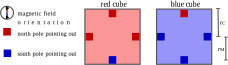
\includegraphics[width=0.75\textwidth]{figures/magnetic_cubes.pdf}
	\caption[Top-down view of the two magnetic modular cube types]{Simplified top-down view of the two magnetic modular cube types with their outward pointing magnet poles, illustrated as red and blue squares. Also visualizes the lengths $r_C$ and $r_M$}
	\label{fig:magnetic_cubes}
\end{figure}

\section{Magnetic Modular Cubes}
The magnetic modular cubes are cube-shaped bodies embedded with permanent magnets on the four side faces.
The magnets have different orientations of their north and south pole. 
One pole is always pointing outside and the other straight to the center of the cube.
The magnet at the front face has its north pole pointing outwards and the magnet at the back its south pole.
These two magnets ensure that the cube is always aligned with the global magnetic field and this orientation holds true for both cube types.
The two other side faces must have the same outwards pointing pole, so that it is not possible for this axis to align with the magnetic field.

In fact, this is the reason a distinct definition of front, back and side is even possible.
Since the front is always pointing to the north pole of the magnetic field, we also call it the north face, or north edge in two dimensions, and all the other faces can also be called by their corresponding cardinal direction.
For each face we define a vector $\vec{e} \in \{ \vec{N},\vec{E},\vec{S},\vec{W}\}$ with $\lVert \vec{e} \rVert = 1$ pointing the the cardinal direction of the magnetic field.
For simplification we call magnets by their outwards pointing pole in further sections.

Furthermore, two different cube types are defined:
Either both side magnets point out their north pole, these cubes are called red cubes, or they point out their south pole, which is then called a blue cube.
\autoref{fig:magnetic_cubes} shows a top-down view of the two cube types with all the outwards pointing magnet poles.
A compass always shows the orientation of the magnetic field in our illustrations.

Magnetic Modular Cubes can be constructed in different sizes and ways. For more technical details and length measurements, we refer to the original \cite{Bhattacharjee2022}.
Two important lengths that we use for planning and simulating are the cube radius $r_C$ and the magnet radius $r_M$ (also illustrated in \autoref{fig:magnetic_cubes}).
$r_C$ is one half-length of a cube face and $r_M$ is the distance from the center of the cube to the center of the magnet.

\begin{figure}
	\centering
	\includegraphics[width=0.53\textwidth]{figures/workspace_config.png}
	\caption[Workspace with a configuration of four magnetic modular cubes]{Rectangular workspace with a configuration of four magnetic modular cubes. All cubes have the same orientation as the magnetic field, indicated by the compass in the top-left corner.}
	\label{fig:workspace_config}
\end{figure}

\section{Workspace and Configuration}
Magnetic modular cubes could theoretical be placed and maneuvered on any 2-dimensional plane with numerous obstacles, as long as you can surround the workspace with a time varying magnetic field.
The magnetic field should be able to point in any direction specified by angles of latitude and longitude, so that the cubes can operate in all desired motion modes.
Because the motion planning problem of self-assembling target shapes in the special Euclidean group is hard enough without considering obstacles and arbitrary workspace shapes, we only work in a rectangular workspace with no internal obstacles.
The workspace is limited by surrounding walls, which are the only objects that could be considered as obstacles in classical motion planning.
However, we do not assume a fixed size, as long as the workspace stays finite and rectangular.

For planning we work in the configuration space of the 2-dimensional special Euclidean group $SE(2) = \mathbb{R}^2 \times \mathbb{S}^1$.
When only considering one cube, the group consists of the position in $\mathbb{R}^2$ and an orientation $\mathbb{S} = [0,2\pi)$ \cite{LaValle2006}.
When working with $n$ cubes, the dimension of our configuration space increases to $\mathbb{R}^{2n} \times \mathbb{S}^1$.
Note that we can still assume only one orientation for $n$ cubes, because we are working with a global magnetic field orienting all cubes the same way.
\autoref{fig:workspace_config} shows a configuration with four cubes in the workspace.
It is irrelevant which exact physical cube is at which position as long as they are the same type, so switching the positions of the two red cubes in \autoref{fig:workspace_config} would lead to the same configuration as before.

\begin{figure}
	\centering
	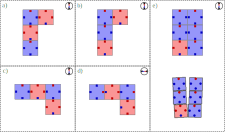
\includegraphics[width=0.65\textwidth]{figures/polyominoes.pdf}
	\caption[Examples of Polyominoes and their equality]{Examples of polyominoes and their equality. a) and d) are equal, only the magnetic field changed its orientation. a) and c) are not equal, they have the same shape but rotated. a) and c) are also not equal because of different cube types in the same shape. e) shows an invalid polyomino in its grid representation (top) and how it behaves in the simulation (bottom).}
	\label{fig:polyominoes}
\end{figure}

\section{Polyominoes}
\label{sec:polys}
The embedded magnets not only align the cube with the magnetic field, they also allow cubes to self-assemble into polyominoes.
Two cube faces can connect if their magnets have opposite polarities.
Because of this and the alignment with the magnetic field, cubes can either be connected at north and south faces, or east and west faces, if the cubes are not the same type.
A polyomino is a set of uniformly sized cubes on a 2-dimensional grid.
Because we work with arbitrary positions and orientations the grid alignment does not hold true for multiple polyominoes in the workspace, but for each polyomino on its own the cubes can be represented in a local coordinate system with position $(x,y)$, $x,y \in \mathbb{Z}$ \cite{Lu2021}.

We consider fixed polyominoes, meaning that two polyominoes are distinct if their shape or orientation are different \cite{Lu2021}.
The magnetic field always provides an orientation, so in \autoref{fig:polyominoes} a) and d) the polyominoes are equal, just the magnetic field is rotated.
Conversely, the polyominoes in \autoref{fig:polyominoes} a) and c) are the same shape but with a different rotation under the same magnetic field orientation, so they are not equal.
Furthermore, two polyominoes are only equal if all the cubes at equal positions are the same type.
The polyominoes in \autoref{fig:polyominoes} a) and b) are not equal because the cube types differ.
It is possible that a workspace contains multiple equal polyominoes.
In that case, we refer to them as being the same polyomino-type, instead of calling them equal, since it is important to differentiate between physical polyominoes with different positions.

The size of a polyomino is the number of cubes it consists of.
Because it is easier to view all structures in the workspace as a polyomino, single cubes are often referred to as trivial polyominoes with size 1.
Although it is not possible to connect cubes of same type at east and west faces, the magnetic modular cubes can assemble structures like the one shown in \autoref{fig:polyominoes} e).
The connection of the bottom two cubes is strong enough to hold the structure together, even though the four blue cubes on the top repel each other.
The resulting polyomino in its grid representation has two east-west connections between cubes the same type and is therefor marked as an invalid polyomino.

\begin{figure}
	\centering
	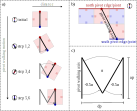
\includegraphics[width=0.80\textwidth]{figures/pivot_walking.pdf}
	\caption[Illustration of the pivot walking motion]{This figure describes the pivot walking motion in detail. a) shows the six pivot walking steps for a single red cube. You can see the orientation of the magnetic field (bigger arrow indicates elevation). In b) an example polyomino with its pivot axis, edges and points is shown. c) illustrates the rotation of the pivot axis labeled with all the pivot walking parameters.}
	\label{fig:pivot_walking}
\end{figure}

\section{Motion Modes}
\label{sec:motion}
In \cite{Bhattacharjee2022} three motion modes are presented. Rotation, pivot walking and rolling.

If the magnetic field orientation lays in the plane of the workspace and rotates without any inclination the rotation is performed around the center of mass for all polyominoes and we consider this motion a normal rotation.

Rotating the magnetic field perpendicular to the workspace plane, cubes can roll forwards or backwards.
This rolling motion becomes problematic for self-assembly, because the top and bottom face of the cube, which contain no magnets, can become a side face.
Because rotation and pivot walking are sufficient to reach any position in the workspace, we do not consider rolling in our simulation and planning algorithms.

When elevating the magnetic field orientation by lifting up the south pole slightly, all polyominoes will pivot on the north face bottom edges of their most north-placed cubes.
Pulling up the north pole does the opposite. The polyominoes will pivot on the south face bottom edges of their most south-placed cubes.
The sum of all these cube edges is called the north or south pivot-edge and by keeping the magnetic field elevated and rotating around the normal vector of the workspace plane, the polyominoes will rotate around the center point of their pivot-edge.
This point is called the north or south pivot-point.
All these edges and points are illustrated in \autoref{fig:pivot_walking} b).

\begin{figure}
	\centering
	\includegraphics[width=0.70\textwidth]{figures/plots/pivot_walking_angle.pdf}
	\caption[Functions of $d_p$ based on $\alpha$ for different $a_p$]{Functions of the pivot walking distance $d_p$ based on pivot walking angle $\alpha$ for different pivot walking axes with length $a_p$. Length are giveen in multiples of cube radius $r_C$.}
	\label{fig:pw_angle_plot}
\end{figure}

\begin{figure}
	\centering
	\includegraphics[width=0.70\textwidth]{figures/displacement_pivot_walking.png}
	\caption[Polyomino shapes with different displacement vectors]{All 19 four-cube polyomino shapes with their displacement vector $\vec{d}$ for one pivot walking cycle with $\alpha = \frac{\pi}{4}$. $\vec{d}$ is drawn from the center of mass (red dot). North and south pivot point are drawn as blue and brown dots.}
	\label{fig:displacement_pivot_walking}
\end{figure}

\paragraph{pivot walking:}
Not rotating around the center of mass is important for pivot walking.
In the first step of a pivot waking cycle, the magnetic field is elevated to let the polyomino pivot on its north pivot edge.
As a second step a rotation of $-\frac{1}{2} \cdot \alpha$ is performed around the north pivot point.
$-\pi \leq \alpha \leq \pi$ is the pivot walking angle.
For step 3 and 4 the elevation changes to its opposite to perform a rotation of $\alpha$ around the south pivot point.
Step 5 and 6 are equal to 1 and 2 and will bring the polyomino back to its original orientation.
You can see the pivot walking cycle steps in \autoref{fig:pivot_walking} a) and have a closer look at its parameters in \autoref{fig:pivot_walking} c).

After one pivot walking cycle, the polyomino has moved by a displacement vector $\vec{d}$ with $\lVert \vec{d} \rVert = d_p$, so $d_p$ is the distance the polyomino moved.
The direction and length of $\vec{d}$ changes with the shape of the polyomino.
The movement is always perpendicular to the pivot walking axis $\vec{a}$ with $\lVert \vec{a} \rVert = a_p$, which is the vector between the north and the south pivot point, visualized in \autoref{fig:pivot_walking} b).
$d_p$ can be calculated as
\begin{equation}
d_p = 2 \cdot \sin\left(\frac{1}{2} \cdot \alpha \right) \cdot a_p \,.
\end{equation}
\autoref{fig:pw_angle_plot} shows functions for this equation based on $\alpha$ for different $a_p$.
To calculate $\vec{d}$ you can take the perpendicular of $\vec{a}$ and scale it to the length $d_p$.

When a big $\alpha$ is chosen according to amount, $d_p$ becomes also bigger, but the polyomino needs more space to the north and south to perform the rotations.
For better maneuvering smaller values of $\alpha$ are preferable.
There is a strong deviation of length and direction of the displacement for different polyomino shapes.
So doing a pivot walking motion might not move two polyominoes in the same direction.
\autoref{fig:displacement_pivot_walking} shows all 19 four-cube polyomino shapes with their displacement vectors.
There are still two options for pivot walking, depending on a negative or positive value of $\alpha$.
You can walk left, in the direction of the west-faces, or right, in the direction of the east-faces.
Although the polyomino actually moves in the direction of $\vec{d}$, we can still say that for instance a pivot walk right moves to the east, because $\left| \angle \left( \vec{E}, \vec{d} \right) \right| < \frac{\pi}{2}$.
We call these two options the pivot walking direction $\vec{w} \in \{\vec{E}, \vec{W}\}$.

	\chapter{Local Planner}
\label{chap:local}

This chapter is about the local planner that will be used for motion planning on a global scale in \autoref{chap:global}.
Local planning means that the planner only focuses on one concrete task.
The task could be, to develop a plan that moves a polyomino from position $a$ to position $b$, or even simpler, to develop a plan for one pivot walk.
Since on a global scale we consider the problem of self-assembly, we are not really interested in changing positions alone.
To work efficiently with local plans in the global planner, the initial and goal configuration of those plans should differ in the set of polyominoes they contain.
The local planner takes two cubes out of different polyominoes and a valid edge-pair as inputs and attempts to establish a connection.
If a local plan was successful, this guaranties a change of polyominoes in the workspace.

For this the local planner makes use of our simulator from \autoref{chap:sim} in a closed-loop manner, meaning that the state of the simulation can be observed at any time and the actions can be adjusted accordingly.
The local planner observes the position of cubes and polyominoes and works with the distance between them.
It also works with the orientation of cube faces.
In a real application of Magnetic Modular Cubes a camera, able to track cubes in the workspace, could to used to retrieve the necessary information. 

The following sections \ref{sec:connect} to \ref{sec:plan} explain the techniques used in the local planning algorithm of \autoref{sec:local_algo}.

\section{Connecting Polyominoes}
\label{sec:connect}

The two main rules that have to considered when connecting two polyominoes are:
First, cubes can only be connected in the way described in \autoref{sec:polys}, so we can distinguish between east-west and north-south connections
Second, pivot walking (\autoref{sec:motion}) only allows the polyominoes to move left, in the direction on their west faces, or right, in the direction of their east faces.
To move in any arbitrary direction it is necessary to rotate the polyomino, so that the east or west faces point into the desired direction.
Keep in mind that a pivot walking cycle is not always performed in the exact east or west, depending on the polyomino shape.

East-west connections are generally easier to handle.
If we want to connect an east face of polyomino $A$ to a west face of polyomino $B$, $A$ has to walk into the east direction towards $B$, or the other way around.
When $A$ should be connected at an south face of $B$, $A$ can now walk into east or west direction towards $B$, or $B$ could again do the opposite.
A closer look on why these movement directions are important and how all of them can be established at any position is taken in \autoref{sec:align}.

\begin{figure}
	\centering
	\includegraphics[width=0.80\textwidth]{figures/holes.pdf}
	\caption{Tree different examples for connecting polyominoes into holes. a) and b) show one-cube-deep holes (a) east-west and b) north-south). c) illustrates a two-cube-deep east-west hole. The edges to be connected are marked yellow.}
	\label{fig:holes}
\end{figure}

\paragraph{Connecting In Holes:}

Connecting two polyominoes where one of the connection-faces is located inside a hole, is a difficult task in the continuous world.
We differentiate between east-west and north-south located holes.
Furthermore a hole can be of a certain depth measured in multiples of $2 r_C$.
\autoref{fig:holes} shows examples for different holes with different depths.

Connecting into a hole with a depth of more than one times $2 r_C$ is not possible.
For instance, when inserting the blue single cube into the polyomino in \autoref{fig:holes} c), the blue cube would connect with north and south faces of the polyomino before even reaching the full depth of the hole.
But even holes with depth $2 r_C$ are hard to handle.
Inserting into a hole can be done by pivot walking, this would only work for east-west holes, or by letting magnetic forces attract the connection-faces.
Relying on magnetic forces alone seem promising, since it would work for both hole types, but in reality not only the forces of the connection-faces are present.
All the forces between other magnets prevent an easy slide-in.
In our simulator the connection-face will be more attracted or repelled by faces outside the hole, then the once inside.
Pivot walking into east-west holes, even with small values for $\alpha$, has also a high failure rate because of other magnets.
We generally try to avoid local plans that are connecting polyominoes inside holes.  

\section{Aligning Cubes}
\label{sec:align}



\section{Walking And Waiting}
\label{sec:walk_wait}



\section{Plan And Plan-State}
\label{sec:plan}



\section{Local Planning Algorithm}
\label{sec:local_algo}
	\chapter{Global Planner}
\label{chap:global}

The task of the global planner is to assemble a specified target polyomino $\mathcal{T}$ given an initial configuration $g_\textit{init}$.
The configuration-space is explored by executing local plans developed by the local planner from \autoref{chap:local}.
That way, the part of the configuration-space we can actually explore is limited to configurations where a connection attempt between two cubes was made.
Compared to $SE(2)$ this part is manageable in size and only contains configurations which are relevant for self-assembly.

Determining how these configurations are explored affects the run time considerably.
Using rapidly-exploring random trees (RRTs) \cite{lavalle1998} yields good results in many cases, since the configuration-space gets evenly explored without the challenge of determining what decisions are promising for the end goal.
But it also explores many configurations which are not necessary for reaching the goal.
For us this approach is not reasonable. 
Because of the high fidelity simulation we are working with, the computation time for a local plan is huge, so planning the assembly of $\mathcal{T}$ with as few local plans as possible is the aim for our global planner.

We need to make well-thought-through connection decisions, that are valid for assembling $\mathcal{T}$, meaning some sort of building plan for a polyomino is needed.
Creating a building sequences by removing one tile at a time from the target was done by Becker et al.\ \cite{Becker2020}.
However, this does not consider sub-assemblies, so all cubes that are not to be connected have to stay separated at any time.

It is hard to prevent sub-assemblies with magnetic cubes following the rules of tilt, so our approach uses an enumeration of ways to cut a polyomino into two parts (\autoref{sec:twocutting}), which will be used for generating a so-called two-cut-sub-assembly graph (\autoref{sec:tcsa}).
This graph functions as a building instruction along side the exploration of the configuration-space.
\autoref{sec:connect_options} provides a closer look on the use of the graph for decision making and \autoref{sec:local_in_global} explains the usage of the local planner on a global scale. 
Finally \autoref{sec:global_algo} combines previous techniques to a global planning algorithm.
For the algorithm the number of cubes in the workspace is limited to the size of $\mathcal{T}$.
An explanation on why is this done and why the problem becomes more complex when working with extra cubes, is provided in \autoref{sec:more_cubes}.


\section{Two-Cutting Polyominoes}
\label{sec:twocutting}

\begin{figure}
	\centering
	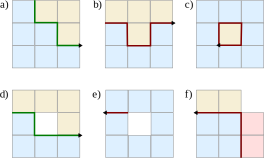
\includegraphics[width=0.6\textwidth]{figures/twocuts.pdf}
	\caption[Different cuts for polyomino shapes]{Examples for cutting polyomino shapes. a) to d) show three two-cuts for a $3\times3$ shape, of which only a) and d) are monotone and therefore valid. b) creates a cave and c) one a hole. e) and f) show cuts that do not split the polyomino into two pieces. e) does not break the polyomino at all and f) creates three sub-polyominoes.}
	\label{fig:twocuts}
\end{figure}

Schmidt et al.\ \cite{Schmidt2018} made use of straight-line two-cuts, to handle the construction of a polyomino with more than trivial sub-assemblies.

We define a two-cut as a continuous edge path through a polyomino that would divide the polyomino into two sub-polyominoes, if all connections with these edges are removed.
For later use in \autoref{sec:tcsa} we want to enumerate all two-cuts of a polyomino that are useful for planning.
We do not limit the cuts by only allowing straight paths like \cite{Schmidt2018}, instead we only consider monotone two-cuts.

\textit{Monotone} means that whenever the path goes into a direction it can never go into the opposite direction again.
\autoref{fig:twocuts} a) shows a monotone two-cut through a $3\times3$ polyomino shape.
The cut starts at the top of the shape and only moves down and right.
By removing all the connections on the path, the polyomino shape is split into two pieces.
Considering non-monotone two-cuts would create sub-assemblies with caves or holes, which could not be reassembled with our local planner.
For this reason they are omitted on a global scale in advance.
\autoref{fig:twocuts} b) shows a non-monotone two-cut creating a cave and \autoref{fig:twocuts} c) one creating a hole.

To calculate all two-cuts of a polyomino, we take all possible monotone paths from each connection as a starting point.
A path ends when it breaks out of the polyomino.
After the path ended the connection at its edges are removed from the polyomino and the path is added as a two-cut, if the polyomino got split into exactly two pieces.
\autoref{fig:twocuts} e) and f) show cuts that split the polyomino in less or more than two pieces.

% 32 possibilities for 3x3

\section{Two-Cut-Sub-Assembly Graph}
\label{sec:tcsa}

\begin{figure}
	\centering
	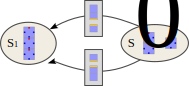
\includegraphics[width=0.45\textwidth]{figures/tcsa_multiedge.pdf}
	\caption[Two two-cut-sub-assembly nodes connected with multiple edges.]{Two two-cut-sub-assembly edges connecting the polyomino sets $S_0$ and $S_1$. The weights of the edges differ, since there are two ways to connect the $2\times1$ with the $1\times1$ to create a $3\times1$ polyomino. The connections are illustrated in rectangular boxes placed on the edges.}
	\label{fig:tcsa_multiedge}
\end{figure}

\begin{figure}
	\centering
	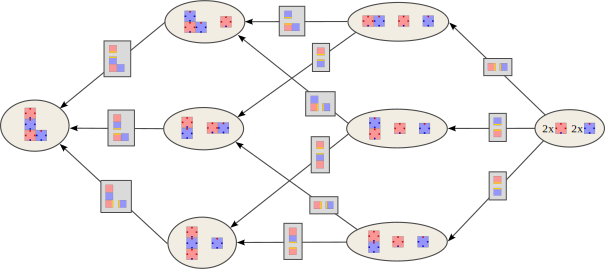
\includegraphics[width=1\textwidth]{figures/tcsa.pdf}
	\caption[Example for a two-cut-sub-assembly graph.]{Example of an two-cut-sub-assembly graph for a four-cube L-shape. The polyomino sets are illustrated as ellipses. If the polyominoes of a set are not numbered, there is only one occurrence of this polyomino. Otherwise the number of occurrences is placed left of the polyomino. The sets are numbered as if the graph was produced by \autoref{algo:build_tcsa} starting from $S_\mathcal{T}$. The weight of edges are illustrated as rectangular boxes containing the polyominoes that need to be connected at specific edges, marked in yellow.}
	\label{fig:tcsa}
\end{figure}
%TODO addglobal plan comic sequence and highlight path in graph

The two-cut-sub-assembly graph, short TCSA graph, functions as a building instruction for a specific target polyomino, we will call it $G_{\textit{TCSA}}(\mathcal{T}) = (V,E)$ represented by nodes $V$ and edges $E$.
The TCSA graph works with sets of polyominoes as nodes.
While a configuration $g$ holds information about orientation and position of physically distinct polyominoes, the corresponding polyomino set $S(g)$ only enumerates the polyomino types preset in $g$.
If $g$ contain multiple polyominoes of the same type, $S(g)$ still stores the amount of the polyomino type, but does not distinguish between the actual polyominoes.

Two nodes $S_0$ and $S_1$ of the TSCA graph are connected with an edge $\{S_0,t_c,S_1\}$, if $S_0$ can be transformed to $S_1$ by connecting two polyominoes contained in $S_0$.
The edge path specifying this connection is stored as the weight $t_c$.
$S_0$ and $S_1$ can be connected by multiple edges, if there are different connections that produce the same outcome.
The edges differ in their weights as shown in \autoref{fig:tcsa_multiedge}.
The direction of $\{S_0,t_c,S_1\}$ always goes from $S_0$ to $S_1$, but we can reverse the definition for an edge as following:

Two nodes $S_0$ and $S_1$ are connected, if one polyomino contained in $S_1$ can be two-cut by an edge path $t_c$, so that the resulting polyomino set equals $S_0$.
This already provides a perspective on the use of two-cuts and the way $G_{\textit{TCSA}}(\mathcal{T})$ is built starting with $\mathcal{T}$.
We will further explain the building process along with an example of a TCSA graph provided in \autoref{fig:tcsa}.


\paragraph{Building a TCSA Graph}

\begin{algorithm}
	\caption{$\text{\scshape Build-TCSA-Graph}$}
	\label{algo:build_tcsa}
	\begin{algorithmic}[1]
		\REQUIRE $\mathcal{T}$ \COMMENT{target polyomino}
		\ENSURE $G_{\textit{TCSA}}(\mathcal{T})$ \COMMENT{the graph is represented by nodes $V$ and edges $E$} 
		\STATE $V \gets \{\}$
		\STATE $E \gets \{\}$
		\STATE $i \gets 0$
		\STATE $V[i] \gets S_\mathcal{T}$ \COMMENT{start with set only containing $\mathcal{T}$}
		\WHILE[work through nodes in BFS manner]{$i < \text{\scshape Size}(V)$}
			\STATE $S_i \gets V[i]$
			\FOR[go through all polyomino types in $S_i$]{\textbf{each} $\mathcal{A} \in S_i$}
				\FOR[go through all monotone two-cuts]{\textbf{each} $t_c \in \text{\scshape Two-Cuts}(\mathcal{A})$}
					\STATE $(\mathcal{A}_1, \mathcal{A}_2) \gets \text{\scshape Cut-Polyomino}(\mathcal{A}, t_c)$
					\STATE $S_\textit{new} \gets \left( S_i \setminus \{\mathcal{A}\} \right) \cup \{\mathcal{A}_1, \mathcal{A}_2\}$ \COMMENT{new node after cutting}
					\IF{$S_\textit{new} \notin V$}
						\STATE $V \gets \text{\scshape Append}(V, S_\textit{new})$
					\ENDIF
					\STATE $E \gets \text{\scshape Append}(E, \{S_\textit{new}, t_c, S_i\})$
				\ENDFOR
			\ENDFOR
			\STATE $i \gets i+1$
		\ENDWHILE
		\RETURN $(V,E)$
	\end{algorithmic}
\end{algorithm}

\autoref{algo:build_tcsa} describes the process of building $G_{\textit{TCSA}}(\mathcal{T})$ for the target $\mathcal{T}$.
The algorithm works through each newly added node in $V$ in a breadth-first-search manner.
The first node added to $V$ is $S_\mathcal{T}$, which is a polyomino set only containing the target shape.

New nodes and edges are determined by two-cutting every polyomino type $\mathcal{A}$ in the current set $S_i$ by every possible monotone two-cut of $\mathcal{A}$.
This is done by enumerating the two-cuts with {\scshape Two-Cuts}, the way it was described in \autoref{sec:twocutting}, and cutting $\mathcal{A}$ at the two-cut with {\scshape Cut-Polyomino}.
The cutting results in the two sub-polyominoes $\mathcal{A}_1$ and $\mathcal{A}_2$.
$S_\textit{new}$ contains the same polyominoes as $S_i$ with the exception that one occurrence of $\mathcal{A}$ is removed and replaced by one occurrence of $\mathcal{A}_1$ and $\mathcal{A}_2$.
Each $S_\textit{new}$ is the result of cutting one polyomino of $S_i$ at a specific two-cut $t_c$.
If $S_\textit{new}$ is not already contained in $V$, we can add it to $V$, which also queues it for future iterations of the breadth-first-search.

No matter if $S_\textit{new}$ is contained in $V$ or not, an edge going from $S_\textit{new}$ to $S_i$ with $t_c$ as the weight is added to the graph edges $E$.
This allow multiple edges, as seen in \autoref{fig:tcsa_multiedge}, and multiple outgoing edges to different nodes, which can be observed in \autoref{fig:tcsa}, where different connections in $S_4$ lead to either $S_1$ or $S_2$.

Each two-cut applied to a polyomino set reduces its amount of polyominoes by one.
Let $n$ be the size of $\mathcal{T}$, then $n-1$ two-cuts applied to $S_\mathcal{T}$ will produce a polyomino set $S_\textit{trivial}$ containing only trivial polyominoes, as it is the case for $S_7$ in \autoref{fig:tcsa}.
All $S_i$ will inevitably end up in this situation and the algorithm will return $(V,E)$, since trivial polyominoes cannot be cut anymore.
This means that no matter which connections are chosen along the way, $n-1$ edges will always be needed to get from $S_\textit{trivial}$ to $S_\mathcal{T}$.
We describe this attribute, by giving the TCSA graph a depth of $n$.
The depth is also illustrated in \autoref{fig:tcsa} and the numbering of the nodes matches the order they were added by \autoref{algo:build_tcsa}.

\subsection{Complexity}

\begin{figure}
	\centering
	\includegraphics[width=0.8\textwidth]{figures/plots/tcsa_nodes_edges.pdf}
	\caption[Average two-cut-sub-assembly nodes and edges for target size $n$.]{Average number of nodes (left) and edges (right) of a TCSA graph for different target sizes $n$. For each $n$ $200$ samples of randomly generated polyominoes were taken. An exponential function is fitted over the averages of nodes and edges.}
	\label{fig:tcsa_plot}
\end{figure}

The Stirling numbers of second kind provide an upper bound for the number of nodes in a TCSA graph.
The Stirling numbers of second kind
\begin{equation}
\bracenom{n}{k} = \sum_{i=1}^{k} \frac{(-1)^{k-i} \, i^{n-1}}{(i-1)! \, (k-1)!}
\end{equation}
describe the possibilities of sorting a set with $n$ objects into $k$ partitions \cite{jelliss1991}.
In our case $n$ equals the target size $n$ and the number of partitions $k$ is the number of polyominoes, the $n$ cubes belong to.
Different layers of depth account for different $\bracenom{n}{k}$.
$S_\mathcal{T}$ is the only polyomino set with $k=1$, so $\bracenom{n}{1} = 1$.
$S_\textit{trival}$ is the only set containing $k=n$ polyominoes, so $\bracenom{n}{n} = 1$.
For the maximum number of nodes possible all layers of the TCSA graph have to be summed up
\begin{equation}
|V|_\textit{worst} = \sum_{k=1}^{n} \bracenom{n}{k} \, ,
\end{equation}
which is also referred to as the Bell number \cite{jelliss1991}.

In our case, the only way of sorting cubes into partitions is by monotonously two-cutting existing polyominoes, which drastically lowers the number of $|V|_\textit{worst}$.
In \autoref{fig:tcsa_plot} statistical data shows the average number of nodes and edges a TCSA graph consists of for varying target sizes $n$.
The growth of nodes and edges seems to be exponential, which is show with fitted functions in \autoref{fig:tcsa_plot}. 

Our implementation of $G_{\textit{TCSA}}(\mathcal{T})$ stores nodes in a hash-table.
Accessing nodes and connected edges, or checking if a polyomino set is contained in $G_{\textit{TCSA}}(\mathcal{T})$, can be done in  $\mathcal{O}(1)$.
The creation of $G_{\textit{TCSA}}(\mathcal{T})$ becomes more complex for increasing numbers of $n$, but it provides an easily accessible building instruction that drastically cuts the number of unnecessary local plans simulated.
Lowering simulation time makes a complex data-structure like the TCSA graph worth the extra effort.


\section{Connection Options}
\label{sec:connect_options}

\begin{figure}
	\centering
	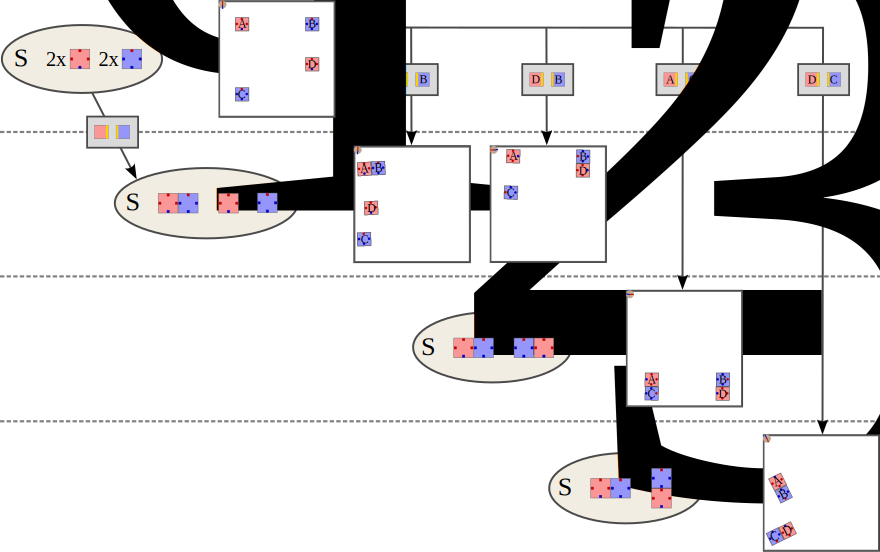
\includegraphics[width=1\textwidth]{figures/connect_options.pdf}
	\caption[Example of connection options for one two-cut-sub-assembly edge]{All connection options when connecting a red cube at the west of a blue cube to get from $S_7$ to $S_4$. Developing a local plan for different polyomino pairs, leads to different goal configurations. $(A_1,B_1)$ and $(A_2,B_1)$ lead to the desired polyomino set $S_4$, but $(A_2,B_2)$ leads directly to $S_2$. All these sets can be found in the TCSA graph of \autoref{fig:tcsa}. The goal configuration of $(A_1, B_2)$ holds the set $S_x$, which cannot be found in \autoref{fig:tcsa}. For further global planning this set could not be used.}
	\label{fig:connect_options}
\end{figure}

In each configuration $g$ the global planner encounters, $G_{\textit{TCSA}}(\mathcal{T})$ will be used to determine the next connection, that the local planner should try to establish.
$G_{\textit{TCSA}}(\mathcal{T})$ will be searched for the node that is the polyomino set $S(g)$.
If $S(g) \notin G_{\textit{TCSA}}(\mathcal{T})$, $g$ cannot be used to assemble $\mathcal{T}$.
This also allows the global planner to state failure immediately, when a initial configuration already contains sub-assemblies that are not usable for assembling $\mathcal{T}$.
With the exception of $S_\mathcal{T}$ all nodes have outgoing edges in a TCSA graph.
All outgoing edges of $S(g)$ provide connections for the local planner that bring the global planner closer to assembling $\mathcal{T}$.

For instance, if $S(g) = S_7$ in \autoref{fig:tcsa}, three outgoing edges provide three connections to choose from, but that is not all.
Assume the global planner decides to connect a red cube at the west edge of a blue cube to end up in a configuration $g_2$ with $S(g_2) = S_4$.
Since $S_7$ contains multiple polyominoes for the same type, there is more than one way to achieve this.
\autoref{fig:connect_options} illustrates all the different connection options for this example case.
You can also see how theses options differ in the goal configurations the local planner ended in.

Let $L_\mathcal{A}$ and $L_\mathcal{B}$ be collections of the physically distinct polyominoes for the polyomino types $\mathcal{A}$ and $\mathcal{B}$.
When $\mathcal{A}$ and $\mathcal{B}$ are about to be connected as the weight of a TCSA edge dictates, there are $\left| L_\mathcal{A} \times L_\mathcal{B} \right|$ polyomino pairs to choose from.
If $\mathcal{A} = \mathcal{B}$, the options where a polyomino will be connected with itself can be eliminated.

With multiple edges and various polyomino pairs per edge, many options emerge for the global planner to consider.
We examined three option sorting strategies for these options, to provide an order of the best probable outcome that the global planner can work through. 
We define functions for determining the best option $\hat{o}$ out of two options $o_1$ and $o_2$.
The approaches are compared in \autoref{chap:results}.

\paragraph{Minimal Distance}

The minimal distance sorting sorts connection options based on the distance between the cubes that are about to be connected.
The idea is that a smaller distances requires less movement to connect, which means shorter simulation time and lower plan costs of the resulting plan.
Due to sliding on walls and different pivot walking distances, this is not true in every case, but it remains a good heuristic for sorting.
Less movement might even prevent unwanted sub-assemblies.
\begin{equation}
\hat{o}(o_1, o_2) =
\begin{cases}
o_1 & \text{if } d(c_{\mathcal{A},1}, c_{\mathcal{B},1}) \leq d(c_{\mathcal{A},2}, c_{\mathcal{B},2}) \\
o_2 & \text{otherwise}
\end{cases}
\end{equation}

\paragraph{Grow Largest Component}

Another approach is to grow the largest component.
The options are sorted into classes of maximum polyomino size $\hat{n}$ of the resulting polyomino set.
We prefer TCSA edges that lead to sets containing the biggest polyominoes.
When the options for $S_4$ in \autoref{fig:tcsa} are sorted, the one leading to $S_1$ is preferred over the one leading to $S_2$, because $S_1$ contains a polyomino of size $3$, while $S_2$ only contains polyominoes of size $2$. 
The options within each class are sorted with the minimal distance approach.

If no other sub-assemblies occur, growing the largest component behaves like one-tile-at-a-time assembly.
The benefit is, that even if they occur the TSCA graph can provide solutions to integrate them if possible.
Larger polyominoes generally move faster acting positive on plan costs.

\begin{equation}
\hat{o}(o_1, o_2) =
\begin{cases}
o_1 & \text{if } \hat{n}_1 > \hat{n}_2 \lor \left( \hat{n}_1 = \hat{n}_2 \land d(c_{\mathcal{A},1}, c_{\mathcal{B},1}) \leq d(c_{\mathcal{A},2}, c_{\mathcal{B},2})\right) \\
o_2 & \text{otherwise}
\end{cases}
\end{equation}

\paragraph{Grow Smallest Component}

Oppositely to growing the largest component, options can be sorted by the smallest maximum size of polyominoes in polyomino sets.
This avoids working with large polyominoes, which are faster, but also need more simulation time to perform rotations and can be hard to handle, because of sheer size.

\begin{equation}
\hat{o}(o_1, o_2) =
\begin{cases}
o_1 & \text{if } \hat{n}_1 < \hat{n}_2 \lor \left( \hat{n}_1 = \hat{n}_2 \land d(c_{\mathcal{A},1}, c_{\mathcal{B},1}) \leq d(c_{\mathcal{A},2}, c_{\mathcal{B},2})\right) \\
o_2 & \text{otherwise}
\end{cases}
\end{equation}

\section{Use of Local Planner}
\label{sec:local_in_global}

The local planner develops plans for connections chosen from the different connection options presented in \autoref{sec:connect_options}.
For the local planner only one connection, out of the path of connections stored in the weight of a TSCA edge, needs to be picked.
Whenever a path consists of both north-south and east-west connections, a north-south connection is preferred.
This is done to perform offset-aligning instead of straight-aligning (\autoref{sec:align}), for an easier slide-in.
Besides of that, the choice of connection is irrelevant, since all connections in the path lead to the same outcome.

When the local planner successfully connects the desired polyominoes, other sub-assemblies can lead to a different polyomino set than expected.
This is not necessarily bad, as long as the resulting set is contained in $G_{\textit{TCSA}}(\mathcal{T})$.
In-fact, more sub-assemblies decrease the number of polyominoes in the workspace, which brings the goal of assembling $\mathcal{T}$ even closer.
Layers of depth were skipped in the TCSA graph, so that it might be possible to assemble $\mathcal{T}$ with less than $n-1$ local plans.
This can be seen in \autoref{fig:connect_options}, where $A_2$ and $B_2$ were connected. 
The resulting polyomino set matches with $S_2$ instead of $S_4$ of the nodes from \autoref{fig:tcsa}.

Like already mentioned in \autoref{sec:connect_options}, when the resulting polyomino set is not in $G_{\textit{TCSA}}(\mathcal{T})$, it is not possible to assemble the target from that configuration.
This can be seen in \autoref{fig:connect_options} when connecting $A_1$ and $B_2$.
For global use we add a new failure condition to the local planner, which checks if the polyomino set of the configuration in the workspace is contained in $G_{\textit{TCSA}}(\mathcal{T})$.
If not, the planner immediately states failure and avoids spending simulation time on a configuration with no further use.

The local planner might even fail to establish the desired connection.
If the resulting polyomino set is contained in $G_{\textit{TCSA}}(\mathcal{T})$, global planning can continue, but there are certain failure types that are not valid for further planning.
Polyomino sets with invalid polyominoes, or where connections in caves are necessary, should not be present in the TCSA graph anyway, but we also do not continue planning with a failure due to maximum movement capacity or polyominoes being stuck.

\section{Global Planning Algorithm}
\label{sec:global_algo}

\begin{algorithm}
	\caption{\scshape Assemble-Target}
	\label{algo:global_algo}
	\begin{algorithmic}[1]
		\REQUIRE $\mathcal{T}$, $g_\textit{init}$ \COMMENT{target polyomino and intital configuration}
		\ENSURE $s$, $P$ \COMMENT{state of global plan $s$ and plan stack $P$ containing local plans}
		\STATE $G_{\textit{TCSA}}(\mathcal{T}) \gets \text{\scshape Build-TCSA-Graph}(\mathcal{T})$
		\STATE $s \gets \text{undefined}$
		\STATE $P \gets \{\}$ 
		\STATE $g \gets g_\textit{init}$ \COMMENT{current configuration $g$}
		\LOOP
			\STATE $O \gets \text{\scshape Connection-Options}(g, G_{\textit{TCSA}}(\mathcal{T}))$
			\STATE valid $\gets$ \FALSE
			\WHILE[try options until local plan is valid]{\NOT $\text{\scshape Empty}(O)$ \AND \NOT valid}
				\STATE $(c_\mathcal{A}, c_\mathcal{B}, e_\mathcal{A}, e_\mathcal{B}) \gets \text{\scshape Pop}(O)$
				\STATE $p_\textit{new} \gets \text{\scshape Local-Planner}(g, (c_\mathcal{A}, c_\mathcal{B}, e_\mathcal{A}, e_\mathcal{B}), G_{\textit{TCSA}}(\mathcal{T}))$
				\IF{$\text{\scshape Valid-Plan}(p_\textit{new})$}
					\STATE valid $\gets$ \TRUE
				\ENDIF
			\ENDWHILE
			\IF{valid}
				\STATE $P \gets \text{\scshape Push}(P, p_\textit{new})$ \COMMENT{add new plan to plan stack}
				\STATE $g \gets g_\textit{goal}$ of new local plan $p_\textit{new}$ \COMMENT{move to new goal configuration}
				\IF[target got assembled]{$\mathcal{T} \in S(g)$}
					\STATE $s \gets \text{success}$
					\RETURN $(s, P)$
				\ENDIF
			\ELSE
				\IF[no configuration to fall back to]{$\text{\scshape Empty}(P)$}
					\STATE $s \gets \text{failure}$
					\RETURN $(s, P)$
				\ENDIF
				\STATE $p_\textit{pre} \gets \text{\scshape Pop}(P)$ \COMMENT{remove last plan from plan stack}
				\STATE $g \gets g_\textit{init}$ of last local plan $p_\textit{pre}$ \COMMENT{fall back to last initial configuration}
			\ENDIF
		\ENDLOOP
	\end{algorithmic}
\end{algorithm}

The global planning algorithm provided in \autoref{algo:global_algo} takes the initial configuration $g_\textit{init}$ and the target $\mathcal{T}$ as inputs and returns the state of the global plan $s$ and a plan stack $P$ as outputs.
For a successful plan, $P$ contains the local plans leading to the assembly of $\mathcal{T}$.
When concatenating the actions of all the plans in $P$, this creates a sequence of actions, that together form the global plan.
Because the local plans were created by using a TCSA graph, $|P| < n$ holds true (\autoref{sec:local_in_global}).
The reason for $P$ being called a stack is the way it is used in \autoref{algo:global_algo}.
The algorithm explores the configuration-space along $G_{\textit{TCSA}}(\mathcal{T})$ in a depth-first-search manner, which is done in the attempt to get closer to assembling $\mathcal{T}$ each iteration.

The algorithm starts with $g_\textit{init}$ as the current configuration $g$.
At first all the connection options for $g$ are determined with {\scshape Connection-Options} the way it was described in \autoref{sec:connect_options}.
The mechanisem behind this function can be viewed as a hash-map, storing the options as the values for the configuration as the key.
The options need to be determined and sorted, only when it is the first time a configuration is encountered.
The list of connection options $O$ that {\scshape Connection-Options} provides, is only a view on the values stored in the hash-map, meaning that when $O$ is altered, the hash-map is updated as well.
Whenever a connection option is popped from $O$, this option is removed from the hash-map and will therefore never be considered again.
Note that options are stored per configuration $g$, not for the polyomino set $S(g)$.
Two configuration sharing the same polyomino set both have their own lists of connection options.
We traverse the configuration-space with the TCSA graph as a guidance, not the TCSA graph itself.
Nodes in $G_{\textit{TCSA}}(\mathcal{T})$ can be encountered multiple times and will never be eliminated from planning.

Once the list of connection options $O$ is retrieved, the algorithm works through it in the order determined by the option sorting that was applied in advance.
This is done until a valid local plan was found, or no options are left.
{\scshape Local-Planner} uses \autoref{algo:local_algo} to create a local plan $p_\textit{new}$.
It also takes $G_{\textit{TCSA}}(\mathcal{T})$ as an input parameter, to ensure the newly added failure condition, when a configurations polyomino set is not contained in $G_{\textit{TCSA}}(\mathcal{T})$.
The validity of a local plan is evaluated with {\scshape Valid-Plan}.

If a valid local plan was found, $p_\textit{new}$ is pushed on to $P$ and $g$ is set to the goal configuration of $p_\textit{new}$.
When a configuration containing $\mathcal{T}$ is reached, the global plan is successful and the algorithm returns.
On the other hand, if no valid option for $g$ could be found, the algorithm has to fall back to the last visited configuration.
For that the top local plan $p_\textit{pre}$ on $P$ is popped and its initial configuration becomes the new $g$.
Even though $p_\textit{pre}$ was a successful local plan, it led to a dead end and had to be removed from the stack.
If $P$ is empty the current configuration is $g_\textit{init}$.
This means that there is no previously visited configuration the algorithm can fall back to.
In that case the algorithm has to state failure for assembling $\mathcal{T}$.

Before calling \autoref{algo:global_algo} checking if $\mathcal{T} \in S(g_\textit{init})$ is necessary, to state early success.
Furthermore, a timeout failure is added to \autoref{algo:global_algo}, in case planning takes to long.
 
\subsection{Complexity}
\label{sec:global_complex}

\paragraph{Optimality}

Given that the local planner does not produce an optimal solution for the connection of two polyominoes, the global planner will also not reach optimality.
Even if the local planner provides only optimal solutions, our depth-first-search approach would not explore the configuration space in a way that the best sequence of local plans is guaranteed to be picked.
\autoref{algo:global_algo} greedily moves along the depth of the TCSA graph to assemble the target as fast as possible.
The option sorting strategies provide reasonable heuristics for picking a connection option per individual TCSA node, but cannot ensure the optimal decision, let alone the optimal decision for the whole path of connection options taken.
Optimal solutions would need broad exploration and comparison of different paths to the target, which is infeasible in our case due to the high simulation time required for local plans.

\paragraph{Completeness}

The same as with optimality, the local planner prevents the completeness of the global planner.
Assuming completeness of the local planner, the global planner could be certain of the existence or non-existence of a solution for assembling $\mathcal{T}$.
\autoref{algo:global_algo} will always return success or failure in finite time.
This is due to the finite number of connection options per configuration and the depth $n$ of the TCSA graph.
Each local plan in the plan stack is certain to connect at least two polyominoes, so after $n-1$ local plans the workspace contains only one $n$-size polyomino.
This polyomino is not necessarily $\mathcal{T}$, but no further connections can be made, which makes the algorithm fall back to the last configuration.
Together with the finite number of options per configuration, the algorithm will eventually explore all paths of connection options that are possible and can therefore verify the existence or non existence of a solution.
Remember that this completeness is based purely on the strong assumption of a complete local planer, which is challenging to archive in the special Euclidean group.

\paragraph{Efficiency}

We have to differentiate between local plans in the plan stack and local plans created during planning $\#\textit{local}$.
Even though $|P| < n$, the global planner might have created more local plans, which were either invalid or had to be removed, because they lead to a dead end.
In a best case only one local plan could lead to the assembly of $\mathcal{T}$.
This is highly unrealistic, but theoretically possible, since layers of depth in the TCSA graph can be skipped.
A more realistic best case would be $n-1$ local plans created during planning. 
This would assume, that all local plans created were valid and lead directly to the target with no layer skipping.

In a worst case all paths of connection options have to be explored before stating failure.
In this worst case ``all'' means that each connection option at each configuration produces a valid local plan with no other sub-assemblies leading to a unique new configuration.
The only invalid local plans are the ones that lead to a configuration with one $n$-size polyomino that is not $\mathcal{T}$.
It is not possible to state the exact amount of worst case local plans, since the number of connection options per configuration varies.
By taking the average number of connection options per TCSA node $o_\mu$, we can define an estimate

\begin{equation}
\#\textit{local}_\textit{worst} = \sum_{i=1}^{n-1} {o_\mu}^i \, .
\end{equation} 
For $n = 10$ and $o_\mu = 20$ this results in $\#\textit{local}_\textit{worst} \approx 5 \cdot 10^{11}$.

It is impossible to simulate that many local plans in a reasonable time.
For that reason a timeout failure was added.
\autoref{chap:results} will provide experimental data on the number of $\#\textit{local}$ and what percentage of global plans time out.
The number of configurations explored $\#\textit{config}$ is also examined in the experiments to better portray the number of dead ends during planning.


\section{More Cubes than Target}
\label{sec:more_cubes}

The number of cubes in the workspace is limited to the target size $n$ for the global planner to work.
The reason for this is linked with the use of TCSA graphs. 
Using a hash-table to find a TCSA node $S_\textit{TCSA}$ and check for equality with the configurations polyomino set $S(g)$ is simple and fast.
If a configuration holds more cubes then the TCSA nodes hold, we need to check if $S_\textit{TCSA} \subseteq S(g)$.
This cannot be done by hash comparing, so all nodes of the graph need to be checked, which would be very costly.
In addition to that, multiple nodes can be included in $S(g)$.
The global planner could handle this by summing up the connection options of all the nodes, but again this makes planning more complex and costly.

After assembling $\mathcal{T}$ all the leftover cubes could assemble various polyominoes.
We could enumerate all possible left over polyomino sets $S_l$ and remove all of them separately from $S(g)$ to check for $S_\textit{TCSA} = S(g) \setminus S_l$.
This would again result in multiple nodes and summed up connection options, but with the ability to hash compare for equality.
The number of $S_l$ can become huge for increasing numbers of leftover cubes leading to a less efficient global planner.





	\chapter{Simulator}
\label{chap:sim}

\begin{figure}
	\centering
	\includegraphics[width=1\textwidth]{figures/simulator_controlflow.pdf}
	\caption[Control flow of the simulator]{long caption...}
	\label{fig:simulator}
\end{figure}

Our simulator used for modeling the behavior of magnetic modular cubes uses the 2d physics library Pymunk\footnote{Pymunk: \url{https://www.pymunk.org/}}.
This library is build for the Python 3 and Python 2 environment based on the 2d physics library Chipmunk\footnote{Chipmunk: \url{http://chipmunk-physics.net/}}.
We used Pymunk, since it can be easily integrated and customized in a Python implementation.
Furthermore it is light-weight and capable of running headless, but also offers an interface for Pygame\footnote{Pygame: \url{https://www.pygame.org/}}, which we use to visualize developed plans and allowing user controls.
As a disadvantage, we are challenge with the simulation of 3d movement in a 2d environment.
That way we trade simulation accuracy for faster simulation time, which is necessary to develop global plans in a reasonable time.

\autoref{fig:simulator} shows a flow chart diagram of the simulators simulation loop.
The diagram provides the control flow of our simulator, where individual steps are explained in this and following sections.

Any control program, in example a local planner or a ``sandbox program'' for visually controlling magnetic modular cubes with keyboard inputs, can interact with the top-level interface of the simulator.
The interface provides functionalities like, starting and stopping the simulation process, controlling the drawing with Pygame, or loading custom configurations and retrieving the current workspace state (\autoref{sec:workspace_state}).
Another crucial functionality is queuing in motions for simulation and notifying the control program, when a motion is done simulating.
After handling the motion control, further explained in \autoref{sec:motion_control}, the simulator enters the Pymunk-step.

The Pymunk-step is a library function, responsible for updating the simulation environment by a certain time step.
The duration of a time step is a parameter that allows adjustment between simulation accuracy and simulation time. 
Inside the Pymunk-step forces are applied to the cubes and collision with workspace boundaries and between cubes is handled (\autoref{sec:coll_handling}).

After the Pymunk-step the magnetic forces between permanent magnets of cubes are calculated, which also determines connections of cube faces used to retrieve information about the polyominoes present in the workspace (\autoref{sec:force_magnet}).
Polyominoes are necessary to calculate the force of the magnetic field acting on cubes (\autoref{sec:force_field}) and friction forces, on which we heavily rely to simulate 3d movement like pivoting on pivot edges (\autoref{sec:force_friction}).
All the calculated forces will be applied in the Pymunk-step in the next iteration of the simulation loop.

When drawing is enabled the Pygame-rendering of the workspace is the last step before beginning the next iteration.

% plot of time use for simulation

\section{Motion Control}
\label{sec:motion_control}

The motion control manages the queued in motions from the control program and determines an update of the magnetic field for each iteration of the simulation loop.
This update consists of the longitude change in radians and the latitude change called the elevation.
In our simulator the elevation just states if the magnetic north points up, the magnetic south points up, or the magnetic field latitude lays in a neutral position within the workspace plane.
We do not specify a angular value of the latitude, since we cannot model it in the 2d-environment anyway.
The elevation just indicates the simulator to simulate pivoting of polyominoes.
More on that in \autoref{sec:force_friction}.

A change of elevation is executed in a single iteration, but the angle of a rotation will be simulated by multiple longitude changes in a linear ramp with a rotational velocity we choose to set to $\frac{\pi}{8} \, \text{rad}/\text{s}$.
Each motion will be simulated by applying its sequence of updates.
After that, the control program is notified.
This makes closed loop control possible by waiting until motions are done.

These updates control the magnetic field orientation and not magnetic modular cubes directly.
Cubes will orient themselves by magnetic field forces we further explain in \autoref{sec:force_field}.
The larger a polyomino is, the more time it needs to align with the magnetic field, which can take longer than rotating the magnetic field itself.
A certain amount of zero-updates is appended to a rotations update sequence depending on the size of the larges polyomino in the workspace.
That way the control program will not be notified until all polyominoes are aligned with the magnetic field.
For this reason simulating larger polyominoes requires more simulation time due to more iterations of the simulation loop.

\section{Workspace State}
\label{sec:workspace_state}

The state of the workspace is stored and updated within the Pymunk-space.
By saving a configuration of the workspace, relevant attributes like position, orientation and velocity of cubes are copied from the Pymunk-space.
These Pymunkt-space attributes will be manipulated when loading in a configuration.

Furthermore a configuration stores magnetic field orientation and the polyominoes, together with their center of mass and pivot points, that got detected by our polyomino detection method elaborated in \autoref{sec:force_magnet}.
Polyominoes are stored in a custom data structure that functions both as a list of physical polyominoes and a polyomino set for the use in two-cut-sub-assembly graphs (\autoref{sec:tcsa}).
The data structure and the polyominoes themselves are hashable for fast equality and inclusion checks.

Individual orientation and velocities of cubes will not be used for planning, but they ensure a correct loading of a workspace configuration that got saved while in motion or when cubes where not or not yet aligned with the magnetic field.
The alignment can be prevented by walls or other cubes, even though we assume perfect alignment with the magnetic field during planning.

\section{Collision Handling}
\label{sec:coll_handling}

Collision is detected and resolved by Pymunk during the Pymunk-step.
For the collision detection Pymunk uses a bounding volume hierarchy of objects in the Pymunk-space.
We also use this efficient collision detection for determining cube pairs in critical-distance.
For that, each cube is surrounded by a circular sensor with half the critical-distance as the radius.
Cubes are in critical-distance if two sensors collide.
Cubes not in critical-distance are to far away to significantly affect each other with magnetic forces of their permanent magnets.
We only calculate magnet forces for cube pairs in critical-distance to speed up simulation.
We set the critical-distance to be $5 r_C$.

\section{Simulating Forces}


% apply with pymunk

\begin{figure}
	\centering
	\includegraphics[width=0.6\textwidth]{figures/plots/magnet_force.pdf}
	\caption[Force between magnets of two cubes for distance.]{long caption...}
	\label{fig:magnet_force}
\end{figure}

\subsection{Magnet Forces}
\label{sec:force_magnet}

% pull cubes together
% provide equation
% plot for magnetic attraction based on distance
% hold cubes together -> polyomino detection
% wich magnetic pairs to choose
% minDist, minDists, all

\subsection{Magnetic Field Forces}
\label{sec:force_field}

% applied to top bottom each indivial cube
% as long as orientation doenst match
% the bigger the poly the longer rotations actually take 
% adding zero updates to motion so that motion finishes when polys oriented


\subsection{Friction Forces}
\label{sec:force_friction}

% force to let poly rotate around pivot point
% splitt friction on cubes on pivot edge
% nominal friction to prevent breaking



	\chapter{Results}
\label{chap:results}

All experiments conducted are about assembling target polyominoes with the use of our global planner (\autoref{chap:global}).
In \autoref{sec:AFN} we analyze the effect of increasing target sizes on planning time, rotational cost and other global planner characteristics mentioned in \autoref{sec:global_complex}.
The polyominoes of this experiment are randomly generated, but we also evaluate the construction of manually designed polyominoes in \autoref{sec:AFTS}.
With these polyominoes, we can specifically test the assembly of targets with caves or holes, varying widths and heights, or different patterns of red and blue cubes. 
Furthermore, we experiment with different workspace sizes and aspect ratios in \autoref{sec:AFBS}.
We run all these experiments with the three option sorting strategies of \autoref{sec:connect_options},
\begin{enumerate}
	\item Minimal Distance (MIN DIST)
	\item Grow Largest Component (GROW LARGEST)
	\item Grow Smallest Component (GROW SMALLEST)
\end{enumerate}

The experiments were done on multiple computers with the same hardware specification (\textbf{AMD Ryzen 7 5800X @ 8x3.8GHz (-4.7 GHz), 128GB RAM}) running Ubuntu 22.04.2 LTS.

For the creation of random polyominoes and initial configurations we used a seed-based pseudorandom number generator to make the experiments reproducible.
That way the option sorting strategies are applied to the same set of seeds to make the results comparable.
The global planner states a timeout failure after a planning time of $600$ seconds.


\section{Assembly for Target Size}
\label{sec:AFN}

This experiment was conducted with randomly generated initial configuration and randomly generated polyominoes of specific target sizes $n$.
To maximize the variety of possible polyomino-shapes the number of red cubes is set to $n_\textit{red} = \lfloor \frac{n}{2} \rfloor$ \cite{Lu2021}.
Because of the variety, this experiment is well-suited for not only analyzing planning time and rotational-cost, but also examine $\#\textit{local}$, $\#\textit{config}$ and $|P|$.
We worked in a quadratic workspace of size $50 r_C \times 50 r_C$ and for each target size $150$ samples were taken.

\paragraph{Time and Failure Analysis}

\begin{figure}
	\centering
	\begin{subfigure}[b]{\textwidth}
		\centering
		\includegraphics[width=0.9\textwidth]{figures/plots/AFN_time.pdf}
		\caption{Planning time in seconds. Only plans that did not time out are shown.}
		\label{fig:AFN_time}
	\end{subfigure}

	\begin{subfigure}[b]{\textwidth}
		\centering
		\includegraphics[width=0.9\textwidth]{figures/plots/AFN_timeout.pdf}
		\caption{Fraction of plans that timed out}
		\label{fig:AFN_timeout}
	\end{subfigure}
	\caption[Planning time and fraction timed out for different target sizes]{Planning time and fraction timed out for different target sizes $n$. All option sorting strategies are compared.}
	\label{fig:AFN_timestats}
\end{figure}



\paragraph{Cost Analysis}

\begin{figure}
	\centering
	\includegraphics[width=0.9\textwidth]{figures/plots/AFN_cost.pdf}
	\caption[Plan cost for different target sizes]{Plan cost of successful plans for different target sizes $n$. All option sorting strategies are compared.}
	\label{fig:AFN_cost}
\end{figure}



\paragraph{Planning Analysis}

\begin{figure}
	\centering
	\begin{subfigure}[b]{\textwidth}
		\centering
		\includegraphics[width=0.9\textwidth]{figures/plots/AFN_nlocal.pdf}
		\caption{Number of simulated local plans.}
		\label{fig:AFN_nlocal}
	\end{subfigure}
	
	\begin{subfigure}[b]{\textwidth}
		\centering
		\includegraphics[width=0.9\textwidth]{figures/plots/AFN_nconfig.pdf}
		\caption{Number of explored configurations}
		\label{fig:AFN_nconfig}
	\end{subfigure}
	\caption[$\#\textit{config}$ and $\#\textit{config}$ for different target sizes]{Number of simulated local plans $\#\textit{local}$ and number of explored configurations $\#\textit{config}$ for different target sizes $n$. All option sorting strategies are compared.}
	\label{fig:AFN_planstats}
\end{figure}

\begin{figure}
	\centering
	\includegraphics[width=0.9\textwidth]{figures/plots/AFN_ltg.pdf}
	\caption[Local plans in plan stack for different target sizes]{Local plans in plan stack $|P|$ for different target sizes $n$. All option sorting strategies are compared.}
	\label{fig:AFN_ltg}
\end{figure}




\section{Assembly for Target Shape}
\label{sec:AFTS}

\begin{figure}
	\centering
	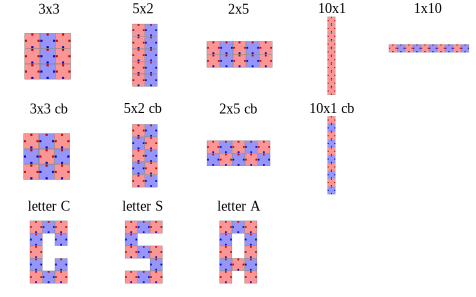
\includegraphics[width=0.8\textwidth]{figures/AFTS_shapes.pdf}
	\caption[List of manually designed polyominoes]{List of manually designed polyominoes for experimenting with special shapes...}
	\label{fig:AFTS_shapes}
\end{figure}


\begin{figure}
	\centering
	\begin{subfigure}[b]{\textwidth}
		\centering
		\includegraphics[width=0.9\textwidth]{figures/plots/AFTS_time.pdf}
		\caption{}
		\label{fig:AFTS_time}
	\end{subfigure}
	
	\begin{subfigure}[b]{\textwidth}
		\centering
		\includegraphics[width=0.9\textwidth]{figures/plots/AFTS_timeout.pdf}
		\caption{}
		\label{fig:AFTS_timeout}
	\end{subfigure}
	\caption[]{}
	\label{fig:AFTS_timestats}
\end{figure}




\section{Assembly for Workspace Size}
\label{sec:AFBS}

\begin{figure}
	\centering
	\begin{subfigure}[b]{\textwidth}
		\centering
		\includegraphics[width=0.9\textwidth]{figures/plots/AFBS_time.pdf}
		\caption{}
		\label{fig:AFBS_time}
	\end{subfigure}
	
	\begin{subfigure}[b]{\textwidth}
		\centering
		\includegraphics[width=0.9\textwidth]{figures/plots/AFBS_timeout.pdf}
		\caption{}
		\label{fig:AFBS_timeout}
	\end{subfigure}
	\caption[]{}
	\label{fig:AFBS_timestats}
\end{figure}

\begin{figure}
	\centering
	\includegraphics[width=0.9\textwidth]{figures/plots/AFBS_cost.pdf}
	\caption[]{}
	\label{fig:AFBS_cost}
\end{figure}




	\chapter{Conclusion}
\label{chap:conclusion}

In this thesis we developed a heuristic approach for the motion planning problem of assembling polyominoes with magnetic modular cubes \cite{Bhattacharjee2022} in the 2-dimensional special Euclidean group $\textit{SE}(2)$.

Although our simulator is not a physically accurate representation of magnetic modular cubes, since we are simulating 3D-movement in a 2D-environment, it is able to depict continuous movement of rotations and pivot walking and also simulates magnetic attraction and repulsion of embedded permanent magnets.
While doing so, collision between cubes and collision with workspace boundaries is detected and resolved.

These attributes of the simulator allow our closed-loop local planning algorithm to dynamically adjust for events like structures blocking each other, structures sliding along the workspace boundaries and varying movement directions due to different pivot walking displacement vectors of polyomino shapes.
By not limiting rotations to certain degrees, structures can always be aligned and theoretically connect by pivot walking a straight path.
Above mentioned events prevent this straight and optimal movement, but dynamic realigning provides a good heuristic for minimizing movement while being efficient on planning time.

We constrained the workspace to be rectangular with no obstacles except the outer boundaries and experimented with different sizes and aspect ratios of the rectangle.
Our local planner is not designed to handle obstacles.
Designing a local planner able to navigate around obstacles and handle pivot walking displacement and sliding on walls in a more calculated way could be a interesting direction for future work.

The simulator is balanced between physical accuracy and efficiency, but it remains a high fidelity physics simulation.
Simulating movement is costly and local plans require planning times in a range of seconds.
On a global scale of doing multiple local plans to assemble desired target structures, simulation should be avoided as much as possible.
Using classical motion planning approaches that broadly explore the configuration-space like RRT, are not feasible under this condition.

Our global planner uses the ability of two-cutting polyominoes to create a two-cut-sub-assembly graph that will be used as a building instruction for target polyominoes.
The configuration-space is explored by depth-first-search traversing this graph, to get closer to the target with each local plan.
The graph leaves multiple options for traversing one edge, because it does not consider workspace position of polyominoes. 
We evaluated three strategies of sorting these options by best probable outcome.

The global planner can identify if the assembly of a target is possible out of any sub-assemblies present in the workspace at any point in time, but requires equal amounts of cubes in the workspace and in the target polyomino.
How to work with more cubes than necessary for the assembly, when two-cut-sub-assembly graphs are used, remains an open question for future work with some insights on the problem given in \autoref{sec:more_cubes}.

We evaluated the assembly of polyominoes with up to 12 cubes in varying shapes and patterns of cube types.
Planning time and timeout failures increase exponentially with the number of cubes, as it is expected with increasing dimensionality of the configuration-space.
We are able to solve the majority of instances in well under $200$ seconds, but certain attributes of polyominoes heavily decrease efficiency of the global planner.
We found out that many connections within a polyomino combined with increasing polyomino width produces especially bad results.

The option sorting strategies seem to perform differently for varying shapes, but we were not able to identify a clear pattern.
Studying attributes of polyominoes and their effect on performance is another possible direction for future work.
Designing new specialized option sorting strategies and determining which on to use, based on the target polyomino, looks promising. 

Using our global planner to calculate motion sequences and applying them to a real workspace of magnetic modular cubes will most likely not result in a successful target assembly, because the mismatch between simulation and the real world is too big.
Instead, the simulator could be replaced by a computer vision-based feedback and control system of the workspace, like the one currently developed by Lu et al.\ \cite{Lu2023}.
Resetting configurations to previous states is not possible in the real world.
Although we are resetting configurations in our global planner, we are already trying to avoid unnecessary simulation as much as possible.
Further optimizing the two-cut-sub-assembly graph traversal to make even more careful decisions could be promising for a real world applications of magnetic modular cubes and actual hardware experiments would be interesting to see.








	
	\bibliographystyle{abbrv}
	\bibliography{bibliography.bib}

\end{document}